\section{Comparing Transfers via Intermediate Sun-Earth Halos to Direct Transfers}
Just like the example tradespace provided in Section 4.3.3 with \cref{fig:tradespace}, for a given
cislunar departure orbit, the "direct" transfers are compared to the staging orbit ones. The
tradespaces for all of the cislunar departure orbits used in this investigation are provided in
Appendix A, along with figures showing the departure orbits themselves, but some are introduced in
this section to facilitate the comparison.

In general, for the scenarios examined in this investigation, transfers with lower times-of-flight
tend to have higher maneuver costs and vice versa. This is not a strict rule, but as shown in the
example of \cref{fig:tradespace}, the transfer points lie mostly in the upper-left and bottom-right
sections of the tradespace. 

In all of the tradespaces computed in this investigation, the blue points representing the "direct"
transfers mostly lie to the left of the red staging orbit transfers but well above the modified
Hohmann transfer baseline. These correspond to direct transfers with lower TOF but much higher
$\Delta v$ compared to the staging orbit transfers. However, there are often some transfers in the
tradespace where the $\Delta v$ lies below the baseline of the modified Hohmann transfer and even
below those of the staging orbit transfers.

\subsection{A Simple Cost Function}
In the example of \cref{fig:tradespace}, the transfer family that directly departs the system
contains the minimum-TOF and minimum-$\Delta v$ solutions. In this specific case, the
minimum-$\Delta v$ solution of the direct transfers has a lower TOF than most of the staging orbit
transfers. However, this is not always the case, as shown in \cref{fig:lowDeltav}. Here, while the
direct transfers still have a lower TOF, the staging orbit transfer family reaches a lower
$\Delta v$. As a result, often a transfer choice needs to be made balancing TOF and maneuver
$\Delta v$ cost. A cost function can help select desirable transfers that balance these two
parameters.

\begin{figure}[ht]
    \centering
    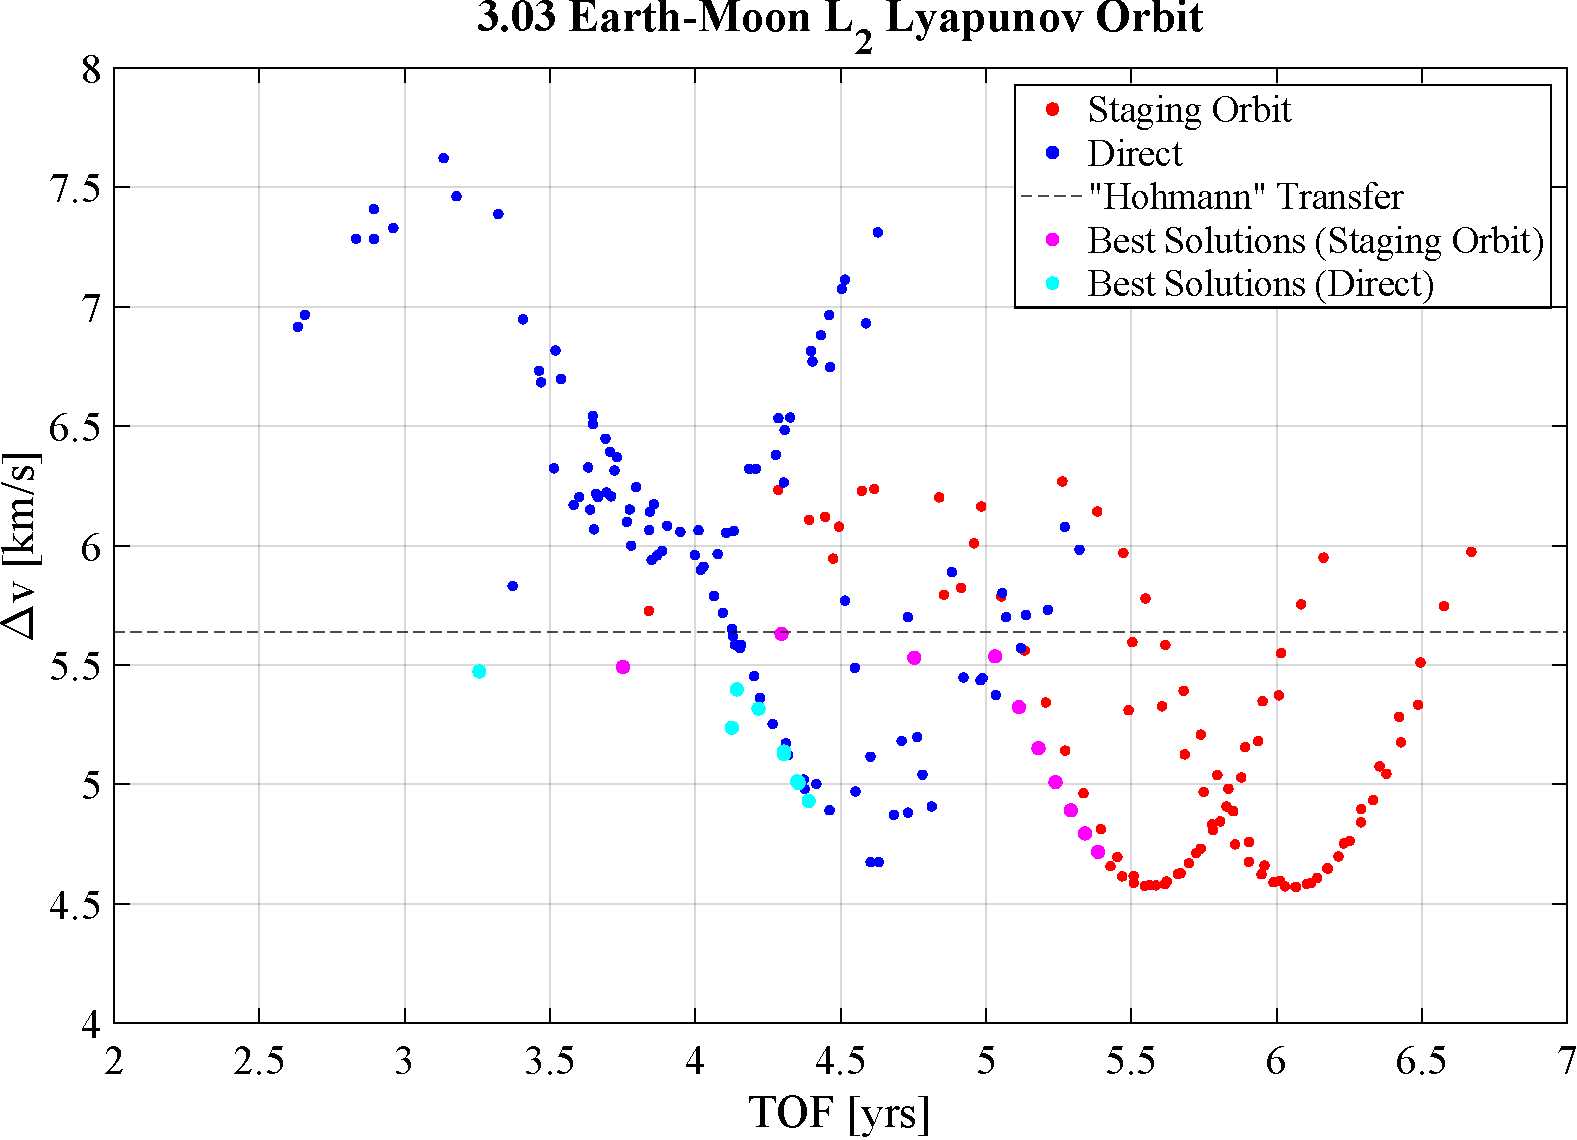
\includegraphics[width=0.75\textwidth]{figures/TradeSpace_L2Lyapunov_3_03.pdf}
    \caption{Transfer tradespace departing from an Earth-Moon $L_{2}$ Lyapunov orbit ($JC=3.03$).}
    \label{fig:lowDeltav}
\end{figure}

If total TOF and total maneuver $\Delta v$ are considered to have units of years and km/s,
respectively, then these values have similar orders of magnitude for these transfers. Therefore, an
appropriate cost function places weights on the two parameters according to the desired transfer
characteristics for a given mission:
\begin{equation}
    J=\alpha TOF+\beta\Delta v,
    \label{eq:costfunction}
\end{equation}
where $J$ is the cost function value and $\alpha$ and $\beta$ are design variables to adjust the
cost function. $\alpha$ and $\beta$ can be adjusted to place higher priority on TOF or $\Delta v$,
depending on the particular application. This investigation uses $\alpha=5$ and $\beta=2$ as a
representative cost function to prioritize lowering the TOF while still looking for decreased
maneuver costs. This cost function is applied to transfers in the tradespace that are below the
modified Hohmann transfer $\Delta v$ baseline, and the ten transfers that have the lowest $J$-value
from each transfer category are determined to be the best transfers for this application. In
\cref{fig:lowDeltav}, these are cyan points for the "direct" transfers and magenta ones for the
"staging orbit" transfers.

\subsection{Comparing Best Cost Solutions between Transfer Types}
In \cref{fig:lowDeltav}, among the best solutions selected using the cost function, the direct
options have a lower average TOF than the staging orbit ones, $4.04$ and $4.94$ years,
respectively, while the transfers with staging orbits achieve a slightly lower average $\Delta v$
cost, $5.207$ km/s compared to $5.238$. The earlier example from \cref{fig:tradespace}, now shown
including the best solutions from the cost function in \cref{fig:costTradespace}, produces similar
results. In contrast, the "direct" options in \cref{fig:lowBoth} have both lower times-of-flight
and maneuver costs when compared to the staging orbit transfers, $4.33$ years and $4.869$ km/s
average for direct transfers versus $4.82$ years and $5.148$ km/s for those with a staging orbit.
In all of the tradespaces computed in this investigation, the best cost direct solutions perform
better than the best cost staging orbit transfers with regards to TOF. While the best staging orbit
solutions often have slightly lower $\Delta v$ costs on average, the significantly longer
times-of-flight outweigh those benefits, and there are still many cases where the direct options
require lower maneuver costs.

\begin{figure}[ht]
    \centering
    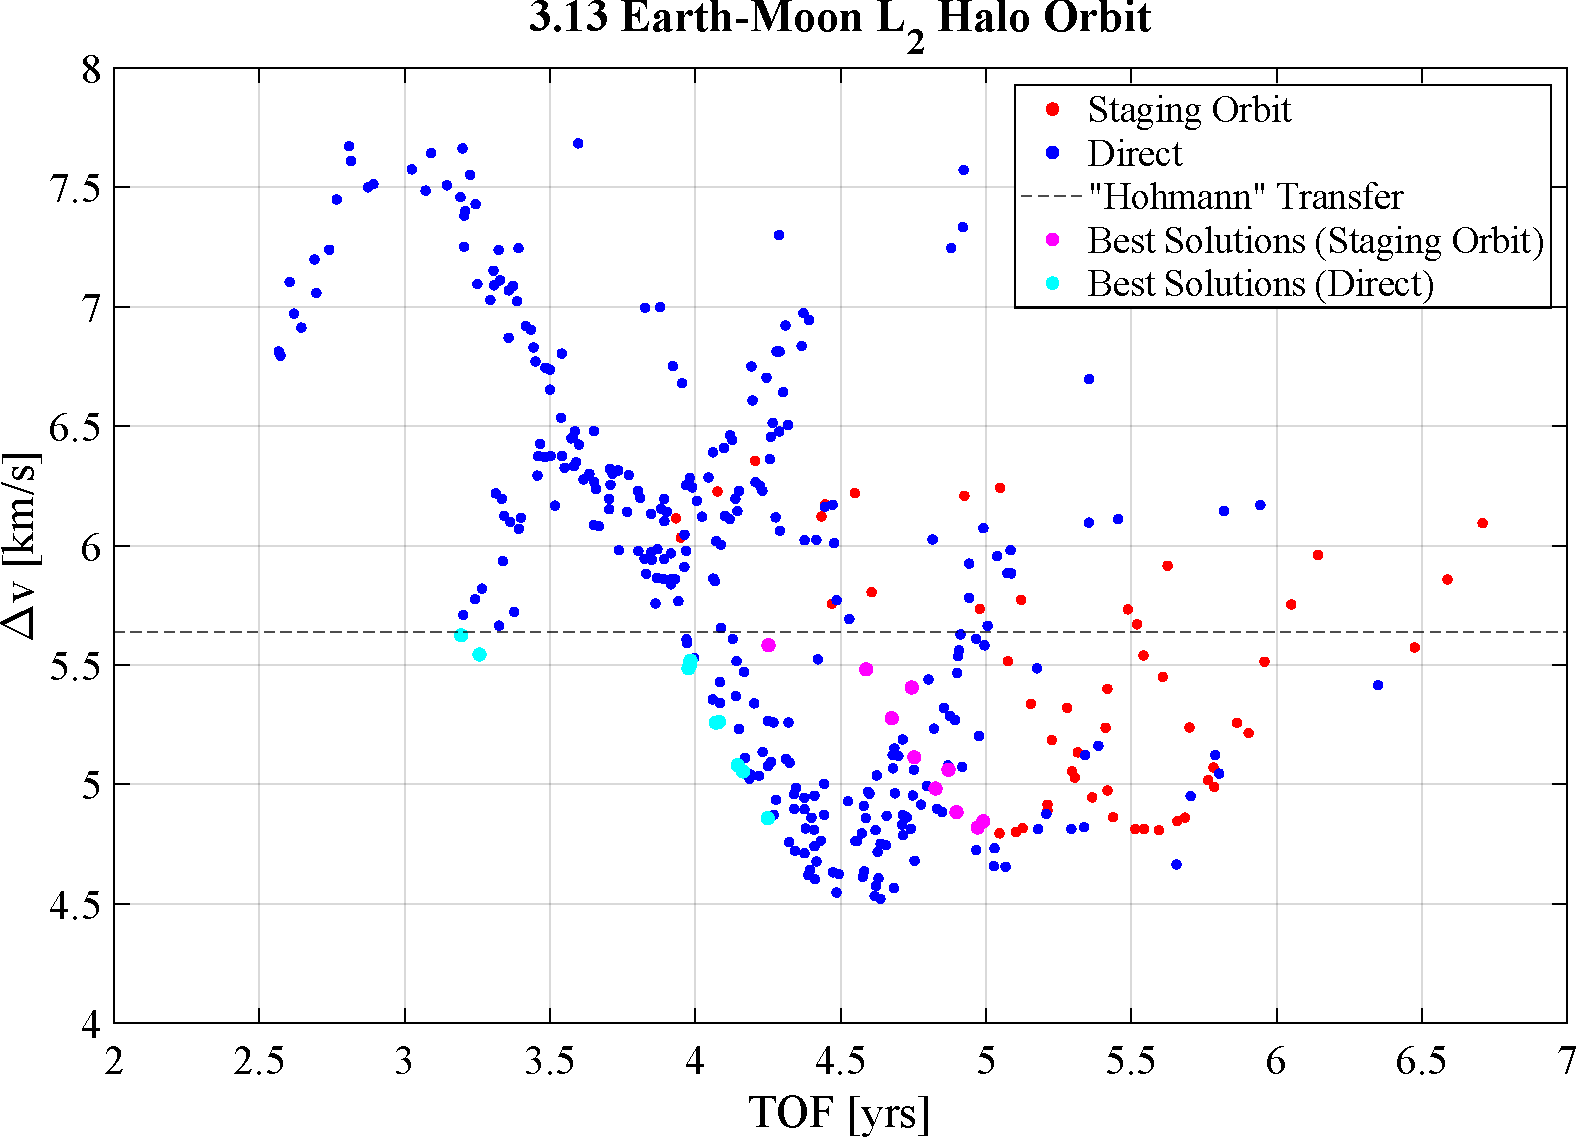
\includegraphics[width=0.75\textwidth]{figures/TradeSpace_L2Halo_3_13.pdf}
    \caption{Transfer tradespace departing from an Earth-Moon $L_{2}$ northern halo orbit ($JC=3.13$).}
    \label{fig:costTradespace}
\end{figure}

\begin{figure}[ht]
    \centering
    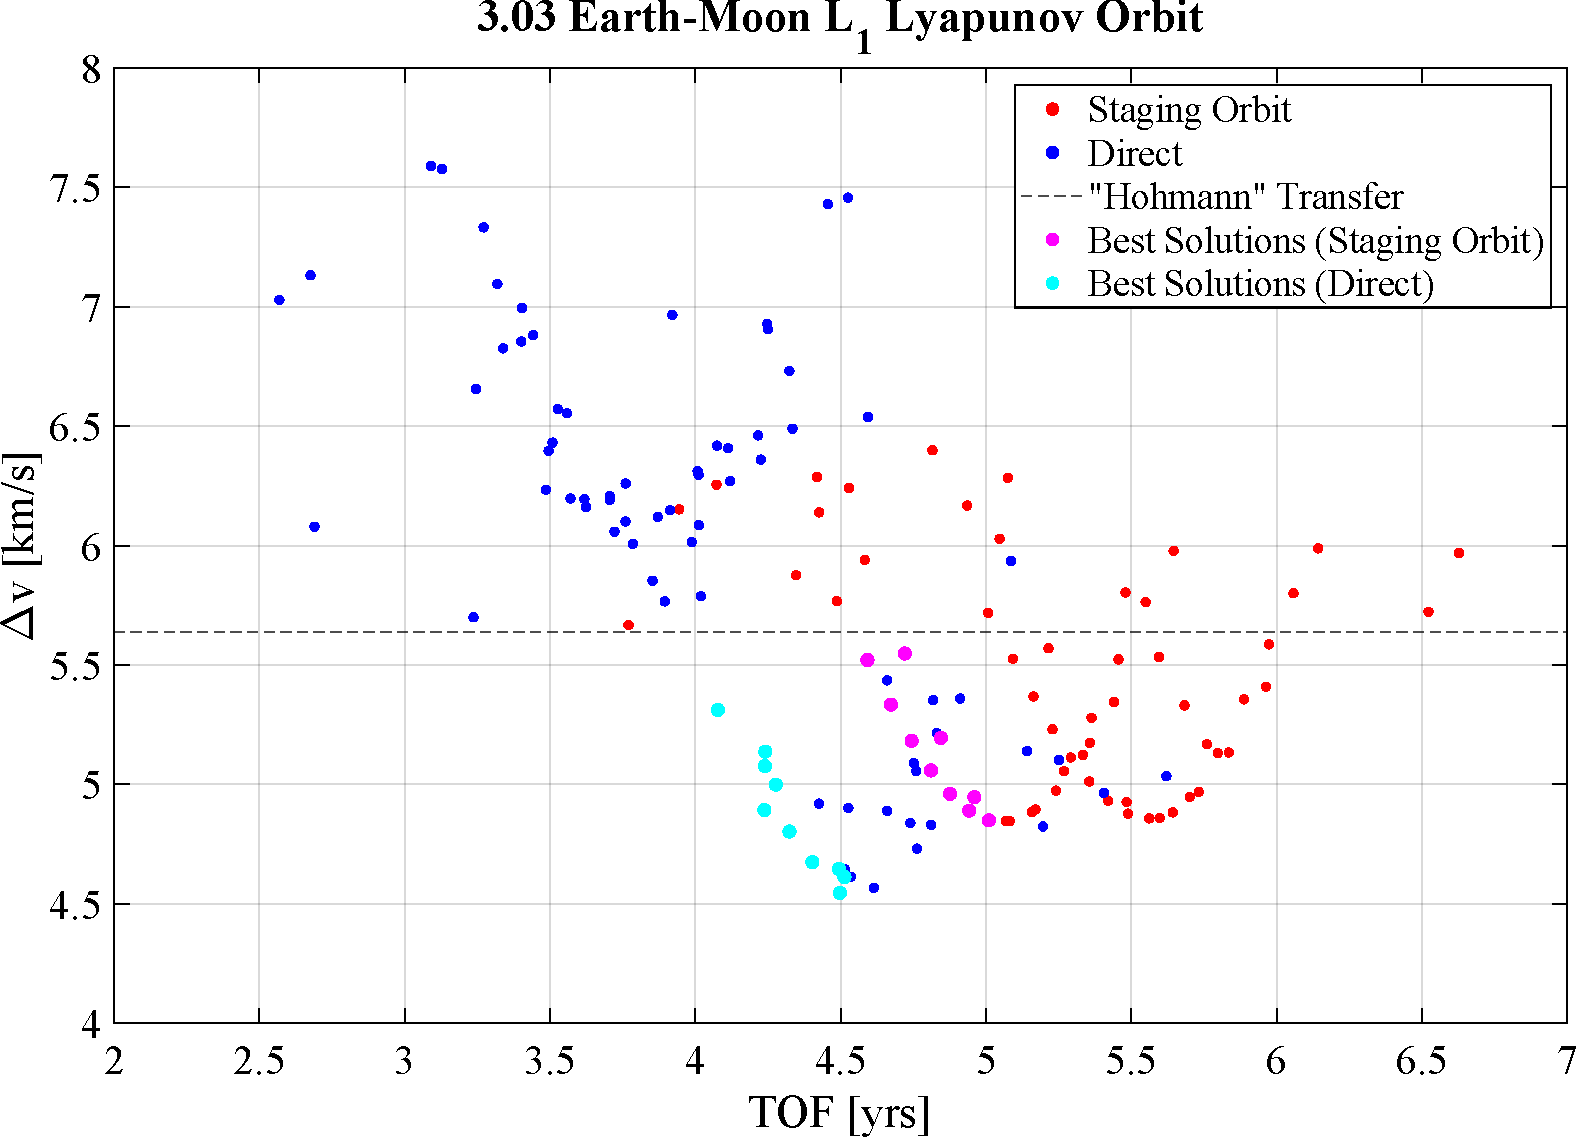
\includegraphics[width=0.75\textwidth]{figures/TradeSpace_L1Lyapunov_3_03.pdf}
    \caption{Transfer tradespace departing from an Earth-Moon $L_{1}$ Lyapunov orbit ($JC=3.03$).}
    \label{fig:lowBoth}
\end{figure}

One downside to the direct departure method is that it relies on the spread and rapid departure of
the Earth-Moon unstable manifolds. A major contributing factor is the cislunar orbit's proximity to
the Moon or Earth. If manifold arcs crash into one of the primaries or get captured by their
gravitational effects, it can delay the arcs' departure from the system and also impact their
distribution in position space, leading to fewer available transfers. The stability of the orbit
also plays a role in affecting the departure time since more unstable orbits have manifolds that
depart the orbit vicinity faster. When there are fewer departure arcs available, it leads to fewer
successful end-to-end transfers with direct departures, as shown in \cref{fig:fewDirect}. Note that
there is a significantly decreased number of available "direct" solutions and that the ones that do
exist no longer follow a familial pattern similar to the previous examples. Since the staging orbit
transfers only require one manifold arc to interface with the Sun-Earth orbit stable manifold,
there is still a full range of staging orbit transfers available for this case. However, the best
cost direct solutions still outperform the staging orbit ones in this specific scenario.

\begin{figure}[ht]
    \centering
    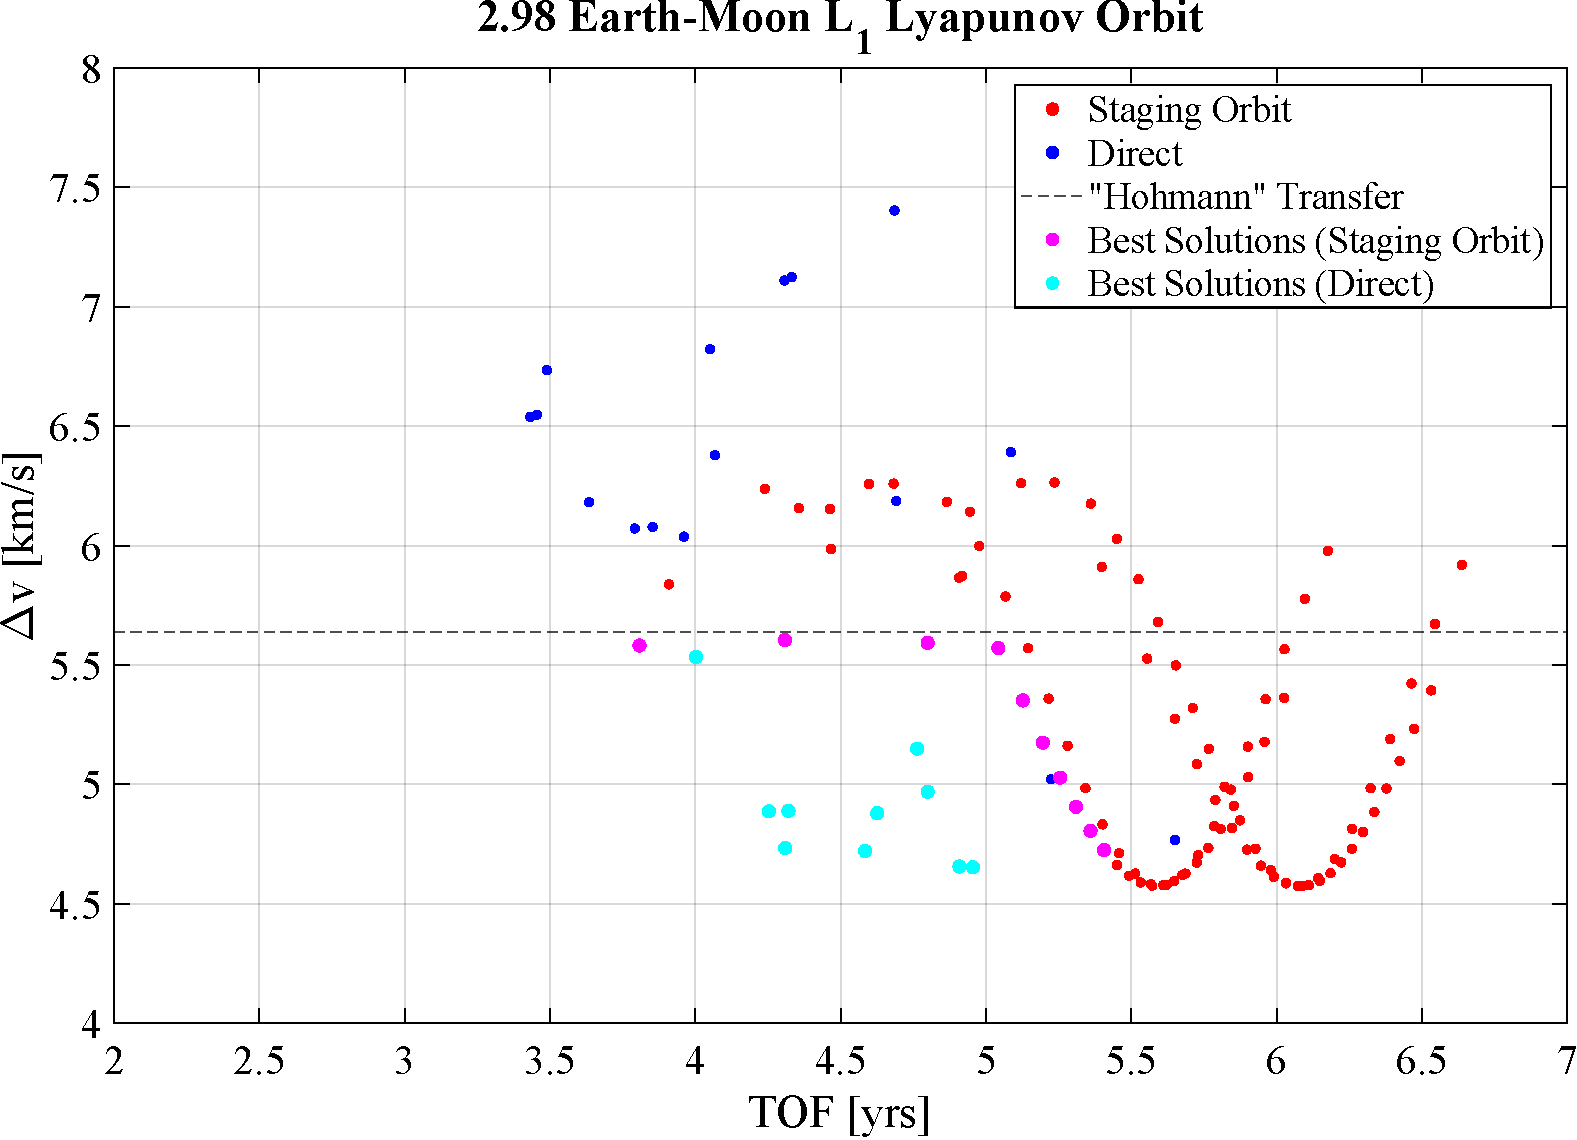
\includegraphics[width=0.75\textwidth]{figures/TradeSpace_L1Lyapunov_2_98.pdf}
    \caption{Transfer tradespace departing from an Earth-Moon $L_{1}$ Lyapunov orbit ($JC=2.98$).}
    \label{fig:fewDirect}
\end{figure}

The results of this investigation and the provided observations demonstrate that the methodology
developed to construct end-to-end cislunar-to-Mars transfers that directly depart the Sun-Earth
system performs better overall than the strategy that incorporates an intermediate Sun-Earth halo
staging orbit. The best cost solutions that directly depart the cislunar orbits used in this
investigation always have a faster average TOF than the best cost staging orbit transfers. While
the direct options only sometimes have a lower $\Delta v$ maneuver cost than the staging orbit
ones, the decrease in TOF is significant enough to outweigh the potential slight increases in
maneuver cost.
